A slice containing all of the elements of the Trigger Processor
design has been implemented with no timing errors and is being tested using a Xilinx VC707
Development board. This board includes a Virtex XC7VX485T-2FFG1761C
FPGA. The implementation includes two ADDC GBT interfaces and associated
trigger processor algorithm.  We are currently working on the timing closure of a full design.

To exercise the trigger processor design we have developed an evaluation board based ADDC
emulator. This design can be used to supply properly formatted ADDC
GBT packets through an optical transmitter as sent from an actual
ADDC. The same ART data used for simulations is being used for hardware
testing. We are also generating pseudo random ART data to test the
GBT communication and timing of packet decoder. A block diagram of the data flow  can be seen in Figure~\ref{fig:artDataStimAE}.

\begin{figure}[h]
 \centering
 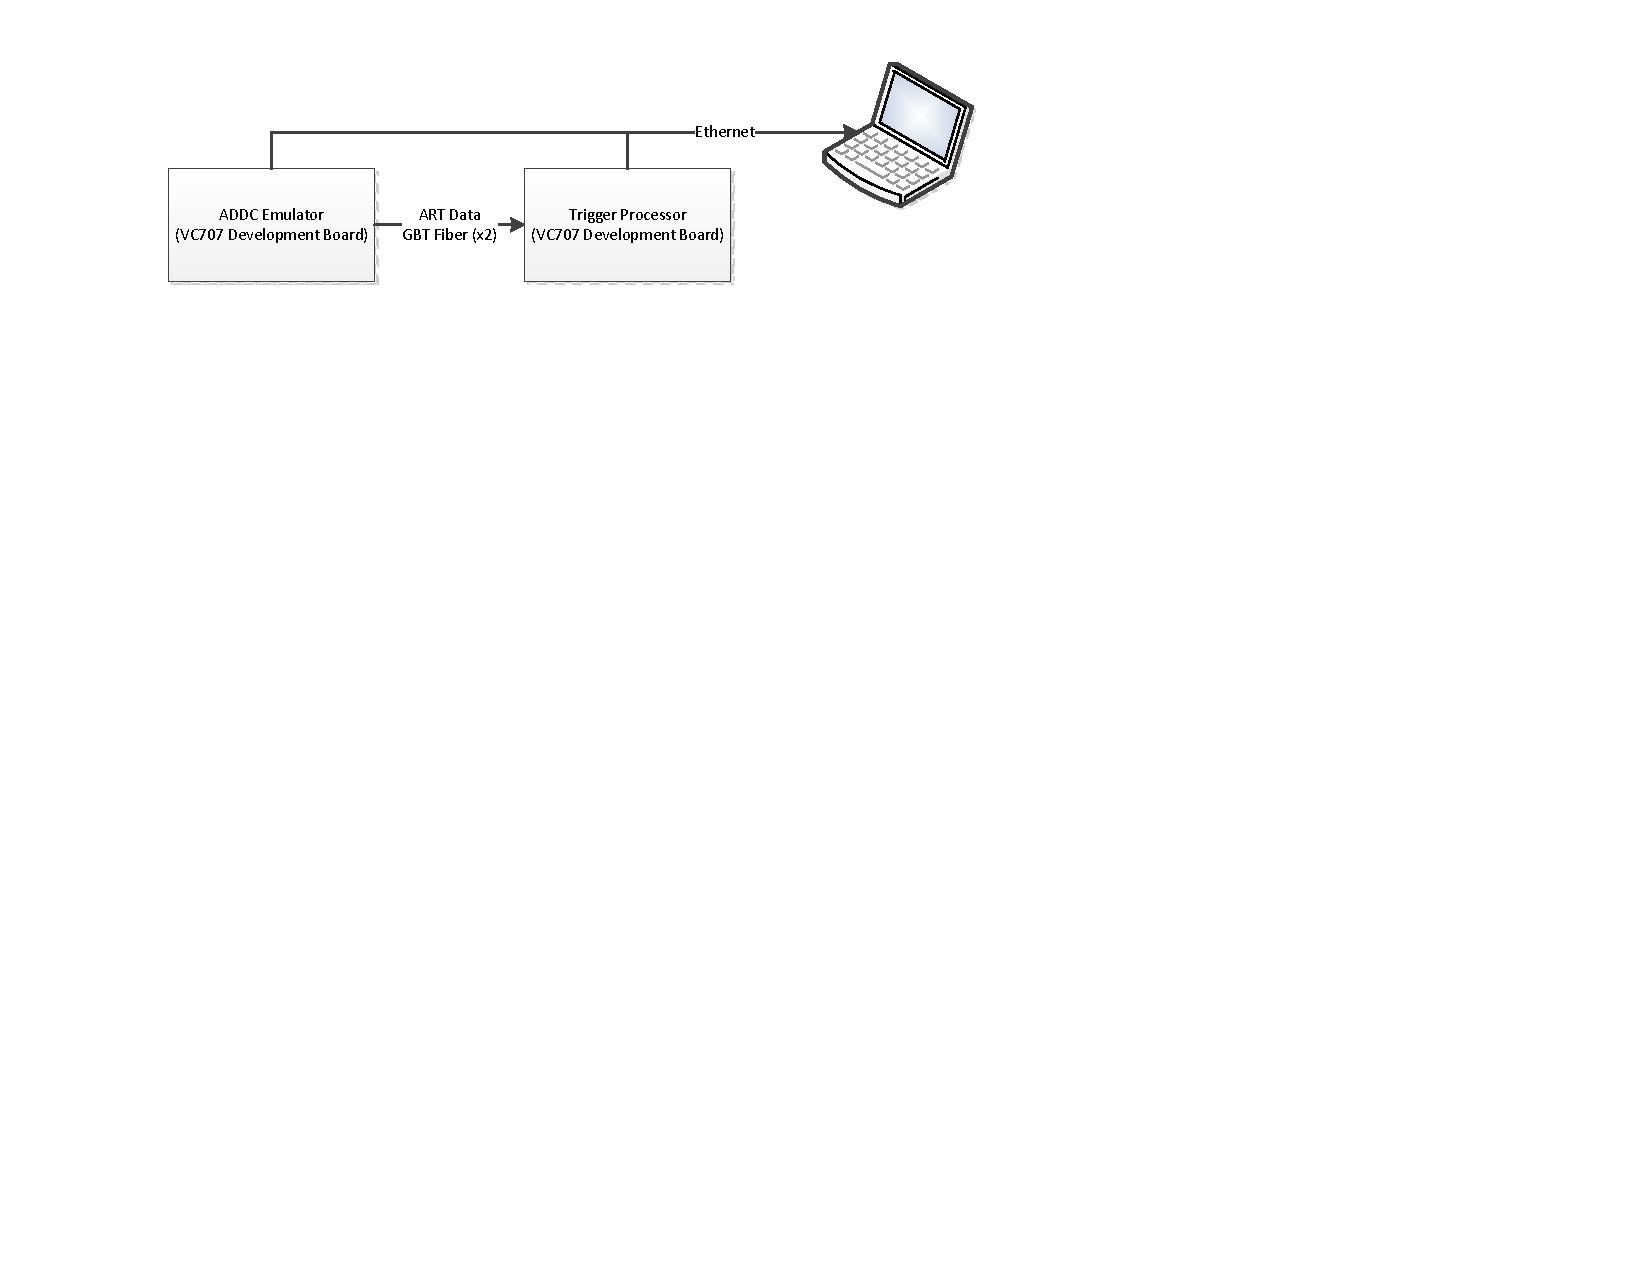
\includegraphics[width=0.7\textwidth]{figures/testing/artDataStimAE.pdf}
 \caption{Initial testing configuration using an ADDC emulator}
 \label{fig:artDataStimAE}
 \end{figure}

To evaluate the hardware implementation, we compare the hardware results
with results generated using a computer simulation of the algorithm. The initial testing of the hardware has shown the entire algorithm is working functionally.  There are some differences between the hardware and software results due to the number of significant bits used in the hardware.  It is likely we will want to increase the precision used in some of the hardware calculations. We expect this would increase the latency by roughly 6 to 9 ns.   Since the calculations are done in an area of the implementation that has a low multiplication factor, increasing the precision will have a low impact on the resources used. 


We have begun integration testing with the BNL ADDC and have successfully
transmitted data to the Trigger Processor using the ADDC's VTTx ASIC.

